% This is "sig-alternate.tex" V2.0 May 2012
% This file should be compiled with V2.5 of "sig-alternate.cls" May 2012
%
% This example file demonstrates the use of the 'sig-alternate.cls'
% V2.5 LaTeX2e document class file. It is for those submitting
% articles to ACM Conference Proceedings WHO DO NOT WISH TO
% STRICTLY ADHERE TO THE SIGS (PUBS-BOARD-ENDORSED) STYLE.
% The 'sig-alternate.cls' file will produce a similar-looking,
% albeit, 'tighter' paper resulting in, invariably, fewer pages.
%
% ----------------------------------------------------------------------------------------------------------------
% This .tex file (and associated .cls V2.5) produces:
%       1) The Permission Statement
%       2) The Conference (location) Info information
%       3) The Copyright Line with ACM data
%       4) NO page numbers
%
% as against the acm_proc_article-sp.cls file which
% DOES NOT produce 1) thru' 3) above.
%
% Using 'sig-alternate.cls' you have control, however, from within
% the source .tex file, over both the CopyrightYear
% (defaulted to 200X) and the ACM Copyright Data
% (defaulted to X-XXXXX-XX-X/XX/XX).
% e.g.
% \CopyrightYear{2007} will cause 2007 to appear in the copyright line.
% \crdata{0-12345-67-8/90/12} will cause 0-12345-67-8/90/12 to appear in the copyright line.
%
% ---------------------------------------------------------------------------------------------------------------
% This .tex source is an example which *does* use
% the .bib file (from which the .bbl file % is produced).
% REMEMBER HOWEVER: After having produced the .bbl file,
% and prior to final submission, you *NEED* to 'insert'
% your .bbl file into your source .tex file so as to provide
% ONE 'self-contained' source file.
%
% ================= IF YOU HAVE QUESTIONS =======================
% Questions regarding the SIGS styles, SIGS policies and
% procedures, Conferences etc. should be sent to
% Adrienne Griscti (griscti@acm.org)
%
% Technical questions _only_ to
% Gerald Murray (murray@hq.acm.org)
% ===============================================================
%
% For tracking purposes - this is V2.0 - May 2012

\documentclass{sig-alternate}
\usepackage{color}
\usepackage[usenames,dvipsnames]{xcolor}
\usepackage{url}

\newcommand{\TODO}[1]{{\color{red} TODO: #1}}
\newcommand{\gametitle}{{\color{RoyalPurple} Dragon Architect Academy}}

\toappear{Submitted for review.}

\begin{document}
%
% --- Author Metadata here ---
%\conferenceinfo{Foundations of Digital Games (FDG)}{2015}
% \pdfinfo{
% /Title ()
% /Author (Aaron Bauer, Eric Butler, Zoran Popovic) 
% /Subject ()
% /Keywords ()
% }
%\CopyrightYear{2007} % Allows default copyright year (20XX) to be over-ridden - IF NEED BE.
%\crdata{0-12345-67-8/90/01}  % Allows default copyright data (0-89791-88-6/97/05) to be over-ridden - IF NEED BE.
% --- End of Author Metadata ---

\title{Visual Programming and Cube-Coding Gooooodtimes}

\numberofauthors{1}
\author{Anonymized}

% \numberofauthors{1} 
% \author{
% \alignauthor
% Aaron Bauer, Eric Butler, Zoran Popovi\'c\\
%        \affaddr{Center for Game Science}\\
%        \affaddr{Computer Science \& Engineering}\\
%        \affaddr{University of Washington}\\
%        \affaddr{Seattle, WA 98195}
%        \email{\{awb, edbutler\}@cs.washington.edu}
% }

\maketitle
\begin{abstract}
    \TODO{Giant wall of text just to fill in the space and get an idea of how long the paper actually is. In this paper we present \gametitle{} which is trying to do some interesting research in CS education. CS education is hard, and also a popular thing to do. Attempts for CS stuff/games usually either approach is as a sequence of challanges/puzzles or a free-for-all sandbox funland. We want to explore combining these two aspects. Our contributions include presenting \gametitle{}, thoroughly describing the unaddressed research problems the space, discussing design challenges encountered attempting to tacke these problems, and initial feedback from players.}
\end{abstract}

% A category with the (minimum) three required fields
\category{K.3.2}{Computers and Education}{Computer and Information Science Education -- Computer science education}

\terms{Design, Human Factors}

\keywords{Game-based learning; computational thinking; programming education}

\section{Introduction}
The past few years have seen many efforts to broaden the reach of computer science education and make it available, and appealing, to more students in more places. 
Many of these projects, including some of the most visible such as Scratch and Code.org's Hour of Code~\cite{codedotorg}, are online programming environments that expose users to basic programming concepts. 
Despite the proliferation of these systems, little work has investigated the design of the structure or content of such systems. 
Comparative studies providing evidence for effective ways of presenting these ideas in this context have been largely absent. 

% As one example, we believe the effects of changes in programming language syntax and semantics on novices need more study. 
% One might ask if there are benefits to evolving the available language elements as a novice progresses, and in which order these elements should become available. 
% What combination of language elements affords beginners the most expressiveness without introducing overwhelming complexity? 
% Another set of questions concern the impact of combining puzzles and an open-ended sandbox. 
% Can puzzles provide sufficient structure and guidance to facilitate productive exploration of a game's concepts in an unstructured sandbox? 
% When and how should the player transition between the two? 
% These and many more topics relating to online programming environments deserve further study, particularly in light of their surging popularity \TODO{footnote about \# of Scratch users/Hour of Code participants?}. 
% In this paper, 

In this paper we present \gametitle{}, an educational game designed to be a tool with which to conduct such studies. 
In \gametitle{}, players use a visual, drag-and-drop programming language to control a dragon in a 3D grid world. 
The visual language is a set of \emph{code blocks} that snap together to form programs. 
The player can move the dragon in three dimensions and have the dragon place and remove cubes of various colors. 
In addition to blocks that control the dragon directly, players can also make use of definite loops and procedures (see Figure~\ref{fig:toolbox}).

\begin{figure}[ht]
  \centering
  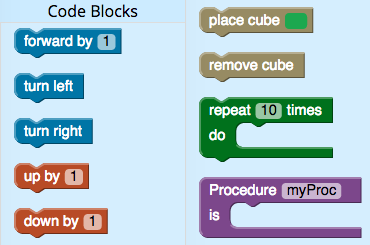
\includegraphics[width=\columnwidth]{images/toolbox_wide}
  \caption{The programming elements currently available in \gametitle{} \TODO{add procedure call block}}
  \label{fig:toolbox}
\end{figure}

Our motivation for developing \gametitle{} is to explore a variety of open questions in both education and games. 
In this paper we review the space of these programming environments and related systems as it currently stands, noting how we differ and how we take inspiration from related work.  
Despite so many existing systems with overlapping educational properties, we developed a new game (as opposed to using existing educational software) in order to design it as a research tool from the ground up.
In Section~\ref{sec:research} we propose four research questions we believe need more study and discuss how these questions have informed the design of our game. 

The remainder of this paper is as follows: after \gametitle{} is described in more detail, it discusses related work and our research goals. 
The paper then highlights several design issues that have arisen during \gametitle{}'s development and presents our observations from students' experiences with the game so far. 
The paper concludes with our thoughts on other interesting questions our game might be used to help answer.

\section{\gametitle{}}
\TODO{Can't use macros in section titles because the formatted gets messed up, replace once we choose a title}
We have been developing \gametitle{} since spring 2014. 
It's played in a web browser, and similar to many other such systems, the page is separated into two parts: an area where the player can assemble their code and a visualization of the environment their code affects (\TODO{figure}). 
The visualization uses the Unity game engine~\TODO{cite} and the drag-and-drop programming UI is provided by the Blockly library~\TODO{cite}.

As they progress through the game, players alternate between short sequences of one to five puzzles with a specific goal and a specific set of available code blocks and an open-ended sandbox. 
The game begins with four puzzles that introduce the idea of assembling and running code, as well as the code blocks for moving the dragon in 2D and putting down cubes.
After that, the player can experiment and build in the sandbox and complete other puzzle sequences to make more code blocks available in the sandbox, switching between sandbox and puzzles at any time. 
Like the first puzzles, each subsequent sequence focuses on a few specific concepts. 
In this way, the language the player uses to write instructions for the dragon gradually expands as the player advances.

\TODO{talk about building on Minecraft's popularity and broad appeal}

% \subsubsection{Language}

% The visual, drag-and-drop language used by the player is a custom, if, in game's development so far, simplistic, language designed specifically for \gametitle{}. We have implemented a textual concrete syntax, and we plan for the game to eventually expose this to the player, allowing them to choose which input method they prefer. This also allows for a direct translation from text to code blocks and vice versa. Some similar projects use a popular industry programming language such as Javascript or Java. We believe implementing our own gives us a valuable flexibility as well as preventing our players from dealing with the idiosyncrasies of any popular language. Having complete control over every part of the language implementation will provide useful in any study of the effects of changes in language features. 

% \subsubsection{Technology}
% \TODO{a few sentences or cut}


\section{Related Work}


\subsubsection{Constructionism}
\emph{Constructionism} is a learning theory that proposes students learn effectively by constructing things of social relevance in a social context \cite{kafai06constructionism}.
Part of constructionism includes theories of discovery learning that suggest students learn best by doing and building.
Another primary aspect of constructionism is that the learning process should occur in a social envionrment in which students are building things that matter to them and the social group.

Others have argued that games are an ideal environment for constructionist teaching \TODO{cite}.
However, evidence suggests that a purely self-directed learning approach is inadquate for effective learning \TODO{cite}.

\subsubsection{Tools and Games for CS Education}
The history of tools designed to teach novices programming dates back to the 1960's, originating with Pappert's LOGO \TODO{cite}.
Kelleher and Pausch review programming environments for novices and describe a taxonomy of these systems~\cite{kelleher2005lowering}.
Within that taxonomy, \gametitle{} fist best as a teaching system that targets \emph{structuring programs} and aims to provide learning support both through \emph{social learning} and \emph{providing a motivating context}.

Lye and Koh recently reviewed studies that investigated teaching \emph{computational thinking}~\cite{wing2008computational} in K12 classrooms~\cite{lye2014review}.
They found that this area deserves more research and that
the reviewed findings suggest structured, guided discovery is a better approach for learning than pure self-driven discovery.



There a been a recent proliferation of widely available CS education tools on the internet.
In some, like the step-by-step lessons available from Khan Academy~\cite{khanacademy} and Codecademy~\cite{codecademy}, or the game CodeSpells \cite{esper2013codespells}, users program in a popular industry programming language such as Javascript or Java.
Given that syntax can be an obstacle for those new to programming~\cite{stefik2013syntax}, other tools chose to use a visual language as there is evidence those are helpful to novices~\cite{whitley1997visual}.
\TODO{should also mention Programming By Design and related project Bootstrap as curricula-oriented projects}
\TODO{cite and talk about AgentSheets}
Examples of such tools include Scratch~\cite{maloney2010scratch}, a visual programming environment focused on empowering its users to create interactive digital media.
Scratch has been successful in building vibrant community around open-ended, creative, social environment (want to borrow ideas of personalization in the future).
Some suggest that the lack of structure may pose a barrier to entry and to learning (quantity and complexity of immediately available features may be intimidating or confusing, discovery-learning-ineffective citation) \TODO{cite};
With \gametitle{}, we want to see if a gradual introduction of features can be easier to get in to while still inspiring the creative experimentation Scratch fostered in its community.

Other recent efforts have, rather than provide an open creative environment, present players with a series of mostly linear challenges.
The game LightBot~\cite{lightbot} asks players to use programming to control a robot in a sequence of linear puzzles. The game has been used to study education in computational thinking~\cite{Gouws13Lightbot}, and is now featured in Code.org's Hour of Code\footnote{\url{http://lightbot.com/hocflash.html}}.
Many of these examples are games, such as Lightbot \TODO{cite} and \TODO{cite some other example}.
Code.org presents a sequence of explanatory videos and linear puzzles. \TODO{cite}
The project has had extremely wide reach but was limited in scope. \TODO{cite}
\emph{BOTS} is a programming puzzle game. The stated goal of the project is to study how community-athored content is used in educational games~\cite{hickspart14}, and it has also been used to explore hint generation~\TODO{cite}.

\subsubsection{Intelligent Tutoring Systems}
Intelligent Tutoring Systems~\cite{koedinger06cognitive} have been successful applied to several teaching domains.
These tutors are typcally rigidly structured, choosing which problem the student will work on next.
These tutors often employ results from cognitive psychology and thus are also called \emph{cognitive tutors}.
Techniques such as Knowledge Tracing~\cite{corbett1994knowledge} model student knowledge with a Bayesian framework.
This modeling requires experts to design a set of \emph{knowledge components} that encompass the skills and abilities players use, as well as a comprehensive set of production rules students use to solve problems in the tutor.
In \gametitle{}, we wish to use direct teaching statagies, but balanced with an open environment in an effort to make the experience more engaging and meaningful to players.
Projects such as \emph{Crystal Island} have integrated ITS technologies into educational games and found success with student knowledge modeling, goal recognition, and affect modeling~\cite{lester2013serious,rowe2010modeling}.
Student modeling is more challenging in games than rigid tutor environments, and this problem is even larger with open-ended games.
Creating a full set of production rules for an open-ended sandbox is not feasible since there are no direct goals.
Even with puzzle sections, creating the set of knowledge components is infeasible for desired concepts such a meta-strategies for programming.

\subsubsection{Minecraft}
Because of the popularity of Minecraft and its ability to engage children, several people have tried to take advantage of this in educational settings.
%Teachers have Here's that project the guy from FDG talked about \TODO{cite}.
%Several people have creating programming plugins for Minecraft
Zorn et al.\ created CodeBlocks, a plugin for Minecraft that allows players to program a robot within the game, and they found that CodeBlocks increased non-programmers' interest in programming~\cite{zorn2013minecraft}.
We wish to draw inpsiration from the aspects that make open multiplayer games like \emph{Minecraft} appealing.
Another avenue people have tried is to teach programming by having students create modifications and plugins for Minecraft, through mods such as ScriptCraft~\footnote{\url{http://scriptcraftjs.org/}}.
Our game does not support mods and instead supports programming as a core mechanic.
\TODO{this could really use some examples of MC-inspired games that aren't \emph{literally} in MC.}


\section{Research Questions}
\label{sec:research}
Our primary goal for \gametitle{} is to produce a flexible system that we can use to investigate questions in computer science education and game-based learning. 
Below we present four questions we believe are under-researched and that informed the design of our game. 

\subsection{Guided Discovery Learning}
Education research indicates that guided discovery, the blending of exploration and direct guidance, can benefit learning
%(see Section~\ref{subsec:learning})
when compared to using just one or the other. 
We believe more research is needed on guided discovery learning in games. 
Some games provide a sandbox where players discover the properties of the environment through largely unguided exploration (e.g. Minecraft, SimCity~\TODO{cite}), and others provide a linear sequence of levels designed to teach the player the relevant information (e.g. Portal~\TODO{cite}). 
In terms of learning theory, the former have a lot in common with pure discovery learning (ignoring potential external sources of information such as wikis or friends), while the latter rely on direct guidance. 

Other games teach players by doing something in between. 
Games in the Zelda series~\TODO{cite} contain a non-linear sequence of puzzles and teach new mechanics by requiring the player demonstrate understanding of a new mechanic before they are allowed to progress. 
Strategy games such as Crusader Kings II~\TODO{cite} offer a set of explicit tutorials the player may choose to go through before beginning more open-ended play.
The variety of approaches games take in teaching players leads to interesting questions about how different methods affect what players do in a game, or, in the case of educational software, how they learn. 
Furthermore, for complex topics such as computer science, the concepts a game needs to teach its players are likely to be more difficult to discover through exploration and require more sophisitcation to explain through direct guidance. Thus, more research is needed to refine and evaluate these techniques. 

In the case of \gametitle{}, we have combined structured puzzle levels and an open, unstructured sandbox. 
The puzzles, by leading the player to demonstrate a particular concept, act as a form of direct guidance. 
A process of discovery can then take place in the sandbox where the player is free to experiment with the ideas introduced in the puzzles. 
As discussed in Section~\ref{sec:action}, our playtesting has shown this to be a promising approach for many of the concepts currently in our game. 

\subsection{Compuational Thinking}

Many have studied (e.g. \cite{barr2011bringing}) how to increase presence of computational thinking in computer science education (and education in general). 
Others have developed games to teach these ideas (e.g. \cite{weintrop2013robobuilder}, \cite{kazimoglu2012serious}). 
Repenning et al.~\cite{repenning2010scalable} report six properties a computational thinking tool for K-12 must have in order to achieve systemic impact. 
In our view, more research is needed to characterize how systems acquire these (and other) useful properties, and what benefits those properties might provide with respect to computational thinking. 

The development of \gametitle{} has been shaped by Wing's~\cite{wing2008computational} definition of computational thinking, which takes automation and abstraction to be its central ideas. 
The open-ended building of our game's sandbox encourages players to take up these principles. 
Since the building must be done via a program written by the player and carried out by their dragon, the player must necessarily automate their ideas. 
As the player sets more sophisticated goals, abstraction becomes important (e.g. abstracting the building of a wall into a procedure) to keep the visual programming feasible. 

We believe there should also be future study on more profound ways to teach computational thinking then simply hoping students absorb this \emph{way of thinking} as a byproduct of working with other computer science concepts (such as basic programming). 
One possible approach (that we explore with \gametitle{}) is to directly teach a core component of computational thinking: the identification and application of problem-solving strategies (in our case, divide and conquer). 
A great deal of recent education research suggests that \emph{curricula can model such strategies for students} and that appropriate guidance, which in many cases consists of the capabilities afforded by a suitable computational environment, can \emph{enable students to learn to use these strategies independently}~\cite{report2010computational}. 
Mayer and Wittrock~\cite{mayer1996handbook} call attention to the substantial evidence in the education literature for teaching what they call \emph{domain-specific thinking skills} and \emph{metacognitive skills}. 
The former would include the ability to use a strategy like divide and conquer, and the latter would include knowing when and where to employ that strategy. 
In both cases, studies have shown that teaching these skills directly can improve learning and performance. 

\TODO{a figure (or two) for this paragraph)}
\gametitle{} explores this with a sequence of puzzles that demonstrate the divide and conquer strategy (i.e. the decomposition of a large problem into smaller subproblems and the subsequent synthesizing of subproblem solutions to solve the original problem). 
The player is presented with a single code block that builds an entire castle, but discovers the construction has a number of flaws. 
The following puzzles each decompose some part of the flawed program in order to give the player a chance to repair it. 
For example, to enable the player to give the castle the correct number of walls and towers, the castle code block is split into a tower block and a wall block that the player uses to write a corrected castle procedure. 
This part of \gametitle{} needs to be expanded and refined before it can be evaluated, but we are confident the larger question merits further attention. 

\subsection{Language for Novices}
For those just starting to program, many aspects of the programming language and programming environment can affect their progress. 
While previous work indicates aspects such as language syntax~\cite{stefik2013syntax}, compiler messages~\cite{nienaltowski2008compiler}, and language semantics~\cite{hoc1990language} can all have an impact, only the first two of those three have been characterized with much specificity. 
Though langauge semantics has certainly been shown to matter for novice programmers, the literature lacks support for more definite conclusions. 
Hence, we see the need for further research on this question to guide the development of programming environments for novices.

This informed our decision to implement a custom language behind \gametitle{}'s visual programming language instead of using a popular existing language like JavaScript. 
Doing so confers several advantages, the first of which is that having complete control over every aspect of the language's implementation gives us the flexibility to experiment widely with langauge semantics. 
In addition, we don't have to inflict the quirks of any existing language on our players. 
Finally, we have implemented a concrete syntax for our language that corresponds precisely with its visual code-block equivalent, so we can expose it to the player and allow them to choose which method of input they prefer. 

\subsection{Social Community}
There are examples where social community has been an important part of the success of an online programming environment. 
Scratch users, for example, have shared millions of projects and even formed online \emph{companies} to tackle projects together~\cite{resnick2009scratch}. 
Research using an online programming environment called MOOSE Crossing~\cite{bruckman1997moose} found that a social context can support and motivate learning programming~\cite{bruckman2000situated}.
This work is supported by research in behavioral and social sciences that indicates sharing and collaboration can improve learning~\cite{bransford2000people}. 
Given these promising results, it is unfortunate the specific contributions of social features to an online programming environment (and how to design those features) remain largely unstudied.

We have incorporated features of this kind into the design of \gametitle{} modeled on the way Scratch lets its users share projects. 
A player can choose to share anything they build in the sandbox, sending it to a gallery containing everyone's shared creations.
Browsing the gallery, players can view, and get the code for, any uploaded construction.
\TODO{we track attribution}

\section{Design Issues}
The design of \gametitle{} has been informed by our research goals, and by existing software such as Minecraft and Scratch. 
In this section we discuss two cases where these objectives presented unusual challenges. 

\subsection{Consistency vs. Experimentation}
Part of Minecraft's popularity is the collaborative multiplayer environment it offers. \TODO{citation, or argument that this is true}
On a Minecraft server, players can explore and shape the world together. \TODO{citation?} 
We want \gametitle{} to be able to provide the same kind of experience, which means giving the world the players inhabit consistency. 
We envision players visiting and admiring each other's constructions or working together on the project. 
While this is relatively straightforward in Minecraft (the whole world shares the same real-time simulation and players' actions are fine-grained with permanent effects), it is complicated in our game by the fact that player input is code. 
Running a single program can have large effects only reversible by tedious effort, so it's important for players to be able to experiment with and tweak their code before committing to it. 
On the other hand, if a player can undo the effects of their programs at will, interactions with existing creations become unpredictable and inconsistent. 

We have so far only partly resolved this tension in \gametitle{}. 
The sandbox makes the effects of programs permanent by default, including any cubes placed and the dragon's position.
To allow for experimentation, the player has the option to switch to \emph{workshop mode}, which resets the world to its previous state each time the player runs a new program. 
The player can freely toggle between these two modes, testing out each program before committing to its results. 
Aside from the fact that the existence of these two modes is difficult to communicate to the player, and that the distinction between them can be confusing, this solution doesn't resolve how to model or visualize the modes in a multiplayer setting. 
Ideally, the player would receive clear indication that effects executed in workshop mode cannot be depended upon.

\subsection{Puzzles as Guidance}
Using puzzles as the guidance in \gametitle{}'s guided discovery is central to the design of the game. 
The puzzles must strike a difficult balance: get the player to the sandbox where they can experiment with their new tools as quickly as possible and support the player in the gradual acquisition of new knowledge and skills. 
Puzzle sequences need to be relatively short to avoid provoking frustration from players who are not engaged by solving puzzles. 

\TODO{this is a super rough idea dump}
Many developers advocate for games with minimal explicit tutorials \TODO{cite}.
Rather than explicitly telling the player how to use new mechanics or tackle particular challenges, games trap players in a limited environment in which they can explore new mechanics in safety and isolation.
This approach to learning in games falls under the category of pure discovery learning.
While it can be extremely effective for certain domains, such as the skills required for an action game, discovery learning performs very poorly when trying to teach metacognitive strageties \TODO{cite}.
As a concrete example in games, it is unlikely that players learn high-level strategies by exploration within the game alone. \TODO{don't really like this example cuz multiplayer, pick a better one. also this isn't rigiorous, also it's bad because you could plausibly learn by studying replays}.
With complex domains, direct guidance is required \TODO{cite} to effectively teach concepts and high-level strategies.

The ideal situation is an open sandbox where just-in-time guidance is given at the most appropriate minute, as an effective human tutor would do.
Intelligent tutoring systems accomplish this by modeling tracking player knowledge and skill.
As we do not have a model for our game domain, this is not an option.

Our current approach is to allow the player unlimited usage of the sandbox and programming tools that they have already used.
In order to unlock new programming tools, player must volunteer to start a new puzzle that will directly guide them in some concept.
A list of available modules advertise what techniques and tools players can learn from puzzles.

However, this approach has several shortcomings.
Emperically in play tests, players have expressed that they wish certain features were available, such as moving the dragon up and down.
In fact, such features were advertised explicitly in the list of modules, but players did not think to check the list, even if they had been there previously.
But even assuming we could get players in the habit of consulting this list, the items they want at the moment was not be obviously on the list.
Perhaps what they do not know how to clearly articulate what the want to do or we as designers have not chosen the best language to describe a techinque.
Then players will not find their desired item on the list.
Human tutors, on the other hand, could help with this translation.

Another problem with this approach is the difficulty in choosing an appropriate sequence of puzzles.
One goal is that players can learn whatever strategy than need to when they need it, with no articifial restrictions gating content.
A contradictory goal is that players are not overwhelmed with concepts at the beginning, as they are in Scratch~\cite{resnick2009scratch} and other fully open tools.
This goal suggest we impose a partial ordering on content and introduce concepts in a deliberate order.
However, with such gating, players may think a feature doesn't exist when, in reality, it's hidden behind several prerequisite concepts.

A potential approach to balance these goals is to expose the entire list of strategies at the start, but still require players to go through the prerequisits.
That is, a player can identify a learning module the wish to reach, and the game will walk them through all the basic skills that they need to get there \TODO{some citation on this style of self-directed learning must exist}.
However, with the entire list was available at the start, seaching for concepts and strategies becomes a more difficult task.

\section{\gametitle{} in Action}
\label{sec:action}
We have conducted numerous playtests since we began developing \gametitle{}, largely with students ages 9 to 14. 
Most had no previous exposure to programming, but some students had previously used systems like Scratch or had participated in the Hour of Code.
Aside from multiple rounds of usability improvements, these playtests gave us insight into \TODO{something}.

A clear message from our playtests is that the premise of programming a dragon in a Minecraft-like world appeals to younger players, and is equally appealing to all genders. 
This is in spite of \gametitle{}'s lack of polish, particularly in the art and UI. 
We have often been asked for a release date or a URL where players can continue with the game. 
Common sandbox activities include making the dragon travel very long distances, building big and impressive towers, and building one's name out of cubes.

We have also noted that building structures in the sandbox is not necessarily the activity of choice for every player. 
Some choose to \emph{doodle} in the sandbox, scattering cubes, often of different colors, in lines and clusters without trying to assemble anything in particular.
Others exclusively seek out the game's puzzles, more interesting in solving those than working in the sandbox.
We believe the freedom a player has to choose what activity interests them most, and to freely switch between them, allows \gametitle{} to engage a wider range of players.

That said, freedom is not always helpful.
Players have gotten \emph{stuck} at the sandbox, unsure of what they should do next, or trying to come up with an idea of what to build. 
We need to more clearly communicate the available options, and provide players ideas to get started with and to use as \emph{jumping off points}.
Other players can also be a source of guidance and ideas, so the social features will play an important role in this as well.

Conceptually, the most common stumbling block we've observed has been a flawed mental model of how the code relates to what the dragon does. 
For example, a player is doing a puzzle where they need to make the dragon move two spaces forward. 
The current program moves the dragon one space forward. 
After running the code, the player sees that the dragon is now only one space away from the goal. 
They quickly reset the program and run it again, not realizing that this resets the dragon as well. 
Another manifestation of this is players add additional code blocks to an existing program, expecting only the new instructions to be run. 
They are surprised when all the code they have assembled is executed. 
Another frequent, if unsurprising, difficulty is procedures. 
Players often don't understand the separation of a procedure into a definition and zero or more invocations. 
This leads to mistakes such as defining a procedure multiple times in order to use it multiple times, or unintentionally introducing recursive calls. 

\TODO{do we need a paragraph to sum up lessons?}

\section{Discussion}
\TODO{description of open problems in CS education and game-based learning, exploration of how \gametitle{} might be used to approach them}
\begin{itemize}
\item visual debugging
\item parallel/distributed programming
\item transition to textual representation
\end{itemize}

% Comment out in submission version
%\section{Acknowledgments}
%\TODO{copy from CHI papers?}

\bibliographystyle{abbrv}
\bibliography{ruthefjord-fdg-2015} 
\end{document}
